% fig1_pipeline.tex  —  System pipeline overview (Fig. 1, teaser)
% Closed-loop quality-aware triage for dermoscopy.
% Compile:  pdflatex fig1_pipeline.tex  (standalone -> fig1_pipeline.pdf)
% Insert:   \includegraphics[width=\textwidth]{figures/fig1_pipeline}
%
% Highlights:
%   C1: DP-Enhance (DP-style enhancement, orange-bordered box)
%   C2: query-for-retake closed loop (bold orange dashed arrow, core novelty)
%
% Colour palette: Okabe-Ito colour-blind friendly
%   Blue   #0072B2  — direct-diagnose channel
%   Orange #E69F00  — enhance-then-diagnose channel  / retake loop
%   Green  #009E73  — cautioned-diagnose channel
%   Red    #D55E00  — retake channel
%   Purple #CC79A7  — input / output nodes
%   Gray   #999999  — shared downstream classifier

\documentclass[tikz,border=4pt]{standalone}

\usepackage{tikz}
\usetikzlibrary{
  arrows.meta,
  positioning,
  fit,
  backgrounds,
  shadows
}
\usepackage{amsmath}
\usepackage{xcolor}
\usepackage{helvet}      % sans-serif: matches LNCS style
\renewcommand{\familydefault}{\sfdefault}

% ── Okabe-Ito palette ──────────────────────────────────────────────────────────
\definecolor{oiBlue}  {HTML}{0072B2}
\definecolor{oiOrange}{HTML}{E69F00}
\definecolor{oiGreen} {HTML}{009E73}
\definecolor{oiRed}   {HTML}{D55E00}
\definecolor{oiPurple}{HTML}{CC79A7}
\definecolor{oiGray}  {HTML}{888888}
\definecolor{oiYellow}{HTML}{F0E442}

% channel fill colours (light tints for node backgrounds)
\definecolor{fillBlue}  {HTML}{D6EAF8}
\definecolor{fillOrange}{HTML}{FEF3CD}
\definecolor{fillGreen} {HTML}{D5F5E3}
\definecolor{fillRed}   {HTML}{FAD7A0}
\definecolor{fillPurple}{HTML}{F5EEF8}

% ── Global TikZ styles ────────────────────────────────────────────────────────
\tikzset{
  % shared base node style
  basenode/.style={
    rectangle, rounded corners=3pt,
    draw, thick,
    minimum width=2.8cm, minimum height=0.75cm,
    align=center, font=\small
  },
  % I/O nodes
  ionode/.style={
    basenode,
    fill=fillPurple, draw=oiPurple, line width=1.2pt
  },
  % central router/decision
  router/.style={
    basenode,
    fill=oiYellow!40, draw=oiOrange, line width=1.4pt,
    minimum width=6.2cm, minimum height=0.9cm,
    font=\small\bfseries
  },
  % channel route boxes (4 colours)
  chBlue/.style={
    basenode, fill=fillBlue, draw=oiBlue, line width=1.2pt
  },
  chOrange/.style={
    basenode, fill=fillOrange, draw=oiOrange, line width=1.4pt
  },
  chRed/.style={
    basenode, fill=fillRed, draw=oiRed, line width=1.2pt
  },
  chGreen/.style={
    basenode, fill=fillGreen, draw=oiGreen, line width=1.2pt
  },
  % shared downstream
  downstream/.style={
    basenode, fill=gray!10, draw=oiGray, line width=1pt,
    minimum width=3.4cm
  },
  % output
  outnode/.style={
    basenode, fill=fillPurple, draw=oiPurple, line width=1.2pt,
    minimum width=3.4cm
  },
  % standard arrows
  arr/.style={-{Stealth[length=5pt,width=4pt]}, thick},
  % channel-coloured arrows (no camelCase, no trailing spaces in key name)
  arr-blue/.style={arr, color=oiBlue},
  arr-orange/.style={arr, color=oiOrange, line width=1.5pt},
  arr-red/.style={arr, color=oiRed},
  arr-green/.style={arr, color=oiGreen},
  arr-gray/.style={arr, color=oiGray},
  % retake loop — bold orange dashed (C2 novelty highlight)
  retake-loop/.style={
    -{Stealth[length=6pt,width=5pt]},
    color=oiOrange, line width=2pt,
    dashed, dash pattern=on 5pt off 3pt
  }
}

\begin{document}
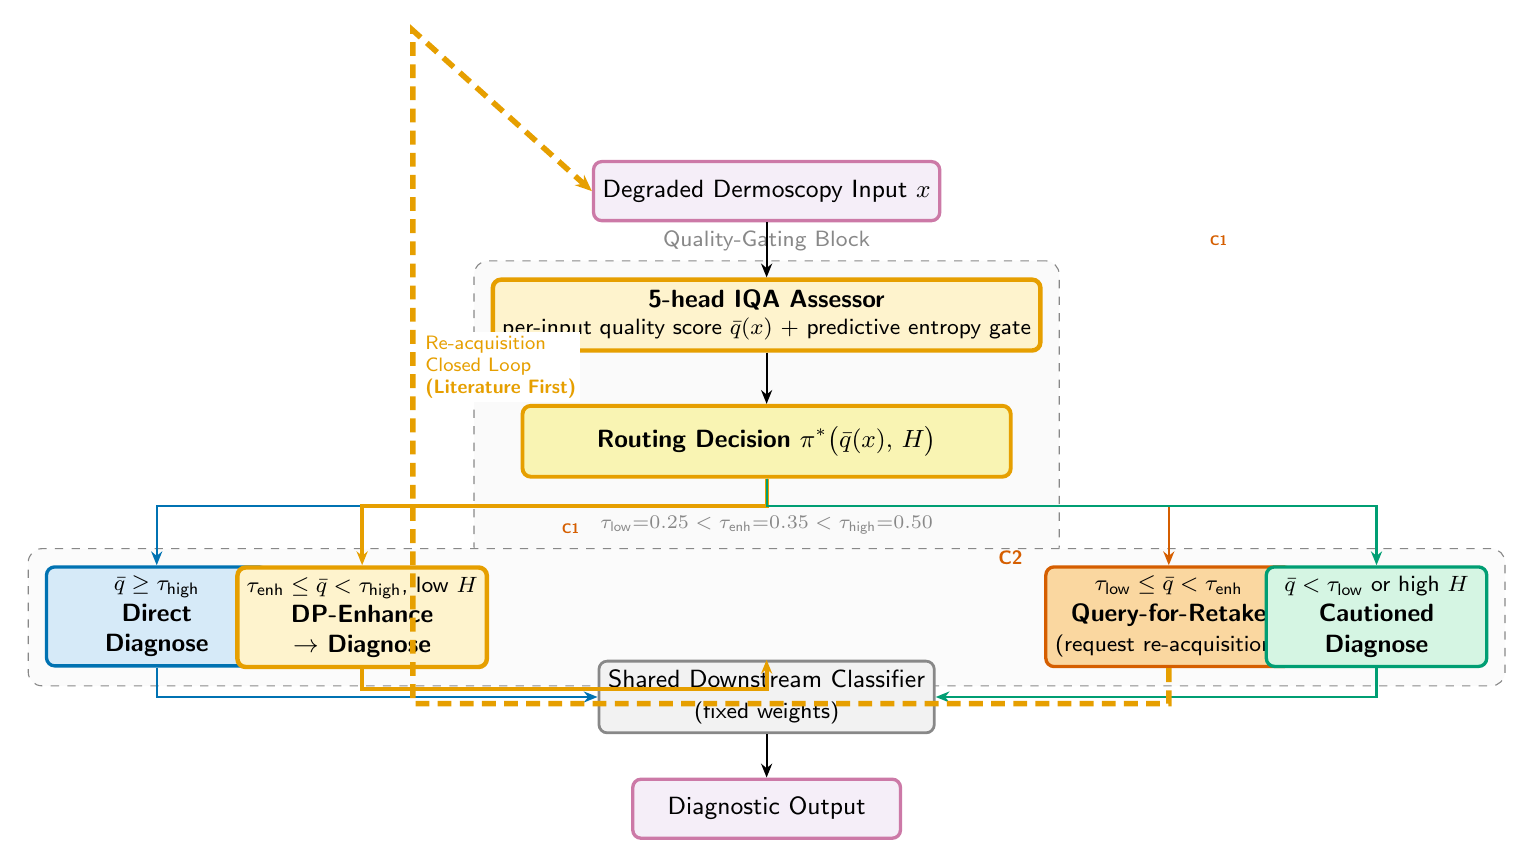
\begin{tikzpicture}[node distance=0.55cm and 0.45cm]

% ─────────────────────────────────────────────────────────────────────────────
%  ROW 0: Input
% ─────────────────────────────────────────────────────────────────────────────
\node[ionode] (input) {%
  Degraded Dermoscopy Input $x$};

% ─────────────────────────────────────────────────────────────────────────────
%  ROW 1: Quality Estimator
% ─────────────────────────────────────────────────────────────────────────────
\node[chOrange, below=0.7cm of input,
      minimum width=6.2cm, minimum height=0.9cm,
      draw=oiOrange, line width=1.6pt,
      label={[font=\tiny\color{oiRed}, xshift=2.0cm, yshift=0.28cm]north east:\textbf{C1}}
      ] (iqa) {%
  \textbf{5-head IQA Assessor}\\[-1pt]
  {\footnotesize per-input quality score $\bar{q}(x)$ + predictive entropy gate}};

% ─────────────────────────────────────────────────────────────────────────────
%  ROW 2: Router
% ─────────────────────────────────────────────────────────────────────────────
\node[router, below=0.65cm of iqa] (router) {%
  Routing Decision $\pi^*\bigl(\bar{q}(x),\,H\bigr)$};

% ─────────────────────────────────────────────────────────────────────────────
%  ROW 3: 4 Channels  (arranged in a horizontal row)
%  Left  → Right:  direct | enhance | retake | cautioned
% ─────────────────────────────────────────────────────────────────────────────

% --- Channel 1: direct diagnose (blue) ---
\node[chBlue,
      below left=1.1cm and 3.2cm of router,
      minimum width=2.8cm, minimum height=1.2cm,
      align=center] (chDir) {%
  {\footnotesize $\bar{q} \ge \tau_\text{high}$}\\
  \textbf{Direct}\\
  \textbf{Diagnose}};

% --- Channel 2: Enhance → Diagnose (orange, C1) ---
\node[chOrange,
      below left=1.1cm and 0.4cm of router,
      minimum width=2.9cm, minimum height=1.2cm,
      draw=oiOrange, line width=1.6pt,
      label={[font=\tiny\color{oiRed}, xshift=0.8cm, yshift=0.28cm]north east:\textbf{C1}},
      align=center] (chEnh) {%
  {\footnotesize $\tau_\text{enh} \le \bar{q} < \tau_\text{high}$, low $H$}\\
  \textbf{DP-Enhance}\\
  $\to$ \textbf{Diagnose}};

% --- Channel 3: query-for-retake (red, C2) ---
\node[chRed,
      below right=1.1cm and 0.4cm of router,
      minimum width=2.9cm, minimum height=1.2cm,
      align=center] (chRetake) {%
  {\footnotesize $\tau_\text{low} \le \bar{q} < \tau_\text{enh}$}\\
  \textbf{Query-for-Retake}\\
  {\footnotesize (request re-acquisition)}};

% --- Channel 4: cautioned diagnose (green) ---
\node[chGreen,
      below right=1.1cm and 3.2cm of router,
      minimum width=2.8cm, minimum height=1.2cm,
      align=center] (chCaut) {%
  {\footnotesize $\bar{q} < \tau_\text{low}$ or high $H$}\\
  \textbf{Cautioned}\\
  \textbf{Diagnose}};

% ─────────────────────────────────────────────────────────────────────────────
%  ROW 4: Shared Classifier
% ─────────────────────────────────────────────────────────────────────────────
\node[downstream,
      below=2.3cm of router] (clf) {%
  Shared Downstream Classifier\\
  {\footnotesize (fixed weights)}};

% ─────────────────────────────────────────────────────────────────────────────
%  ROW 5: Output
% ─────────────────────────────────────────────────────────────────────────────
\node[outnode, below=0.55cm of clf] (output) {%
  Diagnostic Output};

% ─────────────────────────────────────────────────────────────────────────────
%  Threshold annotation strip  (between router and channels)
% ─────────────────────────────────────────────────────────────────────────────
\node[font=\scriptsize, text=oiGray, align=center,
      below=0.35cm of router] (thresh) {%
  $\tau_\text{low}{=}0.25 < \tau_\text{enh}{=}0.35 < \tau_\text{high}{=}0.50$};

% ─────────────────────────────────────────────────────────────────────────────
%  ARROWS — vertical backbone
% ─────────────────────────────────────────────────────────────────────────────
\draw[arr]           (input)  -- (iqa);
\draw[arr]           (iqa)    -- (router);

% router -> channels
\draw[arr-blue]   (router.south) -- ++(0,-0.35) -| (chDir.north);
\draw[arr-orange] (router.south) -- ++(0,-0.35) -| (chEnh.north);
\draw[arr-red]    (router.south) -- ++(0,-0.35) -| (chRetake.north);
\draw[arr-green]  (router.south) -- ++(0,-0.35) -| (chCaut.north);

% channels -> classifier  (blue / orange / green)
\draw[arr-blue]   (chDir.south)    |- (clf.west);
\draw[arr-orange] (chEnh.south)    -- ++(0,-0.25) -| (clf.north);
\draw[arr-green]  (chCaut.south)   |- (clf.east);

% classifier -> output
\draw[arr] (clf) -- (output);

% ─────────────────────────────────────────────────────────────────────────────
%  C2 NOVELTY:  query-for-retake closed-loop arrow
%  Bold orange dashed arc:  chRetake -> left of figure -> back up to input
% ─────────────────────────────────────────────────────────────────────────────
% retake label node (C2 badge)
\node[font=\scriptsize\bfseries, text=oiRed,
      left=0.15cm of chRetake.north west, yshift=0.1cm] (c2badge) {C2};

% The loop path: retake bottom -> go left far -> climb back to input left side
\draw[retake-loop]
  (chRetake.south)
  -- ++(0,-0.45)
  -- ++(-9.6,0)    % go all the way left, past chDir
  -- ++(0, 8.55)   % climb up past router / iqa rows
  node[midway, right=2pt, align=left, font=\scriptsize,
       text=oiOrange, fill=white, inner sep=1.5pt]
       {Re-acquisition\\Closed Loop\\\textbf{(Literature First)}}
  -- (input.west);

% ─────────────────────────────────────────────────────────────────────────────
%  Background grouping panels
% ─────────────────────────────────────────────────────────────────────────────
\begin{scope}[on background layer]
  % IQA + router = "Quality-Gating" panel
  \node[draw=oiGray, fill=gray!4, dashed, rounded corners=5pt,
        fit=(iqa)(router)(thresh),
        inner sep=6pt, label={[font=\footnotesize\color{oiGray}]north:Quality-Gating Block}]
        (gatePanel) {};

  % 4 channels panel
  \node[draw=oiGray, fill=gray!3, dashed, rounded corners=5pt,
        fit=(chDir)(chEnh)(chRetake)(chCaut),
        inner sep=6pt, label={[font=\footnotesize\color{oiGray}]south:Routing Channels}]
        (chPanel) {};
\end{scope}

\end{tikzpicture}
\end{document}
